% Options for packages loaded elsewhere
\PassOptionsToPackage{unicode}{hyperref}
\PassOptionsToPackage{hyphens}{url}
%
\documentclass[
  a4paper,
  oneside,
  open=any]{scrbook}

\usepackage{amsmath,amssymb}
\usepackage{iftex}
\ifPDFTeX
  \usepackage[T1]{fontenc}
  \usepackage[utf8]{inputenc}
  \usepackage{textcomp} % provide euro and other symbols
\else % if luatex or xetex
  \usepackage{unicode-math}
  \defaultfontfeatures{Scale=MatchLowercase}
  \defaultfontfeatures[\rmfamily]{Ligatures=TeX,Scale=1}
\fi
\usepackage{lmodern}
\ifPDFTeX\else  
    % xetex/luatex font selection
    \setmainfont[]{KoPubWorldDotum Light}
\fi
% Use upquote if available, for straight quotes in verbatim environments
\IfFileExists{upquote.sty}{\usepackage{upquote}}{}
\IfFileExists{microtype.sty}{% use microtype if available
  \usepackage[]{microtype}
  \UseMicrotypeSet[protrusion]{basicmath} % disable protrusion for tt fonts
}{}
\makeatletter
\@ifundefined{KOMAClassName}{% if non-KOMA class
  \IfFileExists{parskip.sty}{%
    \usepackage{parskip}
  }{% else
    \setlength{\parindent}{0pt}
    \setlength{\parskip}{6pt plus 2pt minus 1pt}}
}{% if KOMA class
  \KOMAoptions{parskip=half}}
\makeatother
\usepackage{xcolor}
\usepackage[top=30mm,left=25mm,right=25mm,bottom=30mm]{geometry}
\setlength{\emergencystretch}{3em} % prevent overfull lines
\setcounter{secnumdepth}{-\maxdimen} % remove section numbering
% Make \paragraph and \subparagraph free-standing
\makeatletter
\ifx\paragraph\undefined\else
  \let\oldparagraph\paragraph
  \renewcommand{\paragraph}{
    \@ifstar
      \xxxParagraphStar
      \xxxParagraphNoStar
  }
  \newcommand{\xxxParagraphStar}[1]{\oldparagraph*{#1}\mbox{}}
  \newcommand{\xxxParagraphNoStar}[1]{\oldparagraph{#1}\mbox{}}
\fi
\ifx\subparagraph\undefined\else
  \let\oldsubparagraph\subparagraph
  \renewcommand{\subparagraph}{
    \@ifstar
      \xxxSubParagraphStar
      \xxxSubParagraphNoStar
  }
  \newcommand{\xxxSubParagraphStar}[1]{\oldsubparagraph*{#1}\mbox{}}
  \newcommand{\xxxSubParagraphNoStar}[1]{\oldsubparagraph{#1}\mbox{}}
\fi
\makeatother


\providecommand{\tightlist}{%
  \setlength{\itemsep}{0pt}\setlength{\parskip}{0pt}}\usepackage{longtable,booktabs,array}
\usepackage{calc} % for calculating minipage widths
% Correct order of tables after \paragraph or \subparagraph
\usepackage{etoolbox}
\makeatletter
\patchcmd\longtable{\par}{\if@noskipsec\mbox{}\fi\par}{}{}
\makeatother
% Allow footnotes in longtable head/foot
\IfFileExists{footnotehyper.sty}{\usepackage{footnotehyper}}{\usepackage{footnote}}
\makesavenoteenv{longtable}
\usepackage{graphicx}
\makeatletter
\def\maxwidth{\ifdim\Gin@nat@width>\linewidth\linewidth\else\Gin@nat@width\fi}
\def\maxheight{\ifdim\Gin@nat@height>\textheight\textheight\else\Gin@nat@height\fi}
\makeatother
% Scale images if necessary, so that they will not overflow the page
% margins by default, and it is still possible to overwrite the defaults
% using explicit options in \includegraphics[width, height, ...]{}
\setkeys{Gin}{width=\maxwidth,height=\maxheight,keepaspectratio}
% Set default figure placement to htbp
\makeatletter
\def\fps@figure{htbp}
\makeatother
% definitions for citeproc citations
\NewDocumentCommand\citeproctext{}{}
\NewDocumentCommand\citeproc{mm}{%
  \begingroup\def\citeproctext{#2}\cite{#1}\endgroup}
\makeatletter
 % allow citations to break across lines
 \let\@cite@ofmt\@firstofone
 % avoid brackets around text for \cite:
 \def\@biblabel#1{}
 \def\@cite#1#2{{#1\if@tempswa , #2\fi}}
\makeatother
\newlength{\cslhangindent}
\setlength{\cslhangindent}{1.5em}
\newlength{\csllabelwidth}
\setlength{\csllabelwidth}{3em}
\newenvironment{CSLReferences}[2] % #1 hanging-indent, #2 entry-spacing
 {\begin{list}{}{%
  \setlength{\itemindent}{0pt}
  \setlength{\leftmargin}{0pt}
  \setlength{\parsep}{0pt}
  % turn on hanging indent if param 1 is 1
  \ifodd #1
   \setlength{\leftmargin}{\cslhangindent}
   \setlength{\itemindent}{-1\cslhangindent}
  \fi
  % set entry spacing
  \setlength{\itemsep}{#2\baselineskip}}}
 {\end{list}}
\usepackage{calc}
\newcommand{\CSLBlock}[1]{\hfill\break\parbox[t]{\linewidth}{\strut\ignorespaces#1\strut}}
\newcommand{\CSLLeftMargin}[1]{\parbox[t]{\csllabelwidth}{\strut#1\strut}}
\newcommand{\CSLRightInline}[1]{\parbox[t]{\linewidth - \csllabelwidth}{\strut#1\strut}}
\newcommand{\CSLIndent}[1]{\hspace{\cslhangindent}#1}

\usepackage{fontspec}
\setmainfont{KoPubWorldDotum Light}  % Set main body font with fallback
\setsansfont{KoPubWorldBatang Bold}       % Sans-serif font with fallback
\setmonofont{D2Coding}  % Monospaced font with fallback
\usepackage{graphicx}
\usepackage{eso-pic}
\usepackage{lastpage}
\usepackage{wallpaper} % for the background image on title page
\usepackage{fontawesome5}
\usepackage{xcolor}
\let\oldtextbf\textbf
\renewcommand{\textbf}[1]{\textcolor{black}{\oldtextbf{#1}}}
\usepackage{textpos}
\definecolor{orcidlogocol}{rgb}{0.65, 0.807, 0.223}
\definecolor{anugoldtint}{HTML}{F5EDDE}
\definecolor{anugold}{HTML}{BE830E}
\newcommand{\orcid}[1]{\href{https://orcid.org/#1}{\textcolor{orcidlogocol}{\faOrcid} #1}}
\usepackage[manualmark]{scrlayer-scrpage}
\clearpairofpagestyles
\ihead{}
\ofoot{Page \thepage\ of \pageref*{LastPage}}
\ifoot{고려대 노동문제연구소\\{\footnotesize  [02841] 서울특별시 성북구 안암로 145 고려대학교 국제관 121A TEL : 02-3290-1634}}
\addtokomafont{pageheadfoot}{\upshape}

\usepackage{multicol}

\usepackage[most]{tcolorbox}
\newtcolorbox{titlepagebox}{colback=anugoldtint,colframe=white}
\newtcbox{\inlinebox}[1][]{enhanced,
 box align=base,
 nobeforeafter,
 colback=white,
 colframe=gray,
 size=small,
 left=0pt,
 right=0pt,
 boxsep=2pt,
 #1}

% \usepackage{fancyhdr}
% % for title page
% \fancypagestyle{plain}{%
%   \renewcommand{\headrulewidth}{0pt}%
%   \fancyhf{}%
%   \fancyhf[rf]{Page \thepage\ of \pageref*{LastPage}}
% \fancyhf[lf]{The Australian National University\\{\footnotesize TEQSA Provider ID: PRV12002 (Australian University) | CRICOS Provider Code: 00120C}}
% }
% % for other pages
% \pagestyle{fancy}
% \fancyhf{}
% \fancyhf[rf]{Page \thepage\ of \pageref*{LastPage}}
% \fancyhf[lf]{The Australian National University\\{\footnotesize TEQSA Provider ID: PRV12002 (Australian University) | CRICOS Provider Code: 00120C}}
% \renewcommand{\headrulewidth}{0pt} % removes horizontal header line

%\usepackage{titling}
%\pretitle{% add some rules
%   \Huge\bfseries
%}%, make the fonts bigger, make the title (only) bold
%\posttitle{%
% \vskip .75em plus .25em minus .25em% increase the vertical spacing a bit, make this particular glue stretchier
%}

% ensure chapter starts on the same page
\makeatletter
\patchcmd{\scr@startchapter}{\if@openright\cleardoublepage\else\clearpage\fi}{}{}{}
\makeatother
\makeatletter
\@ifpackageloaded{caption}{}{\usepackage{caption}}
\AtBeginDocument{%
\ifdefined\contentsname
  \renewcommand*\contentsname{Table of contents}
\else
  \newcommand\contentsname{Table of contents}
\fi
\ifdefined\listfigurename
  \renewcommand*\listfigurename{List of Figures}
\else
  \newcommand\listfigurename{List of Figures}
\fi
\ifdefined\listtablename
  \renewcommand*\listtablename{List of Tables}
\else
  \newcommand\listtablename{List of Tables}
\fi
\ifdefined\figurename
  \renewcommand*\figurename{Figure}
\else
  \newcommand\figurename{Figure}
\fi
\ifdefined\tablename
  \renewcommand*\tablename{Table}
\else
  \newcommand\tablename{Table}
\fi
}
\@ifpackageloaded{float}{}{\usepackage{float}}
\floatstyle{ruled}
\@ifundefined{c@chapter}{\newfloat{codelisting}{h}{lop}}{\newfloat{codelisting}{h}{lop}[chapter]}
\floatname{codelisting}{Listing}
\newcommand*\listoflistings{\listof{codelisting}{List of Listings}}
\makeatother
\makeatletter
\makeatother
\makeatletter
\@ifpackageloaded{caption}{}{\usepackage{caption}}
\@ifpackageloaded{subcaption}{}{\usepackage{subcaption}}
\makeatother

\ifLuaTeX
  \usepackage{selnolig}  % disable illegal ligatures
\fi
\usepackage{bookmark}

\IfFileExists{xurl.sty}{\usepackage{xurl}}{} % add URL line breaks if available
\urlstyle{same} % disable monospaced font for URLs
\hypersetup{
  pdftitle={국세청 천분위 소득자료(2012-2023)},
  pdfauthor={박영삼},
  pdfkeywords={국세청 천분위 소득자료, 개인소득분배, 불평등, 조세효과},
  hidelinks,
  pdfcreator={LaTeX via pandoc}}


\title{국세청 천분위 소득자료(2012-2023)}
\usepackage{etoolbox}
\makeatletter
\providecommand{\subtitle}[1]{% add subtitle to \maketitle
  \apptocmd{\@title}{\par {\large #1 \par}}{}{}
}
\makeatother
\subtitle{- 통합소득/근로소득/종합소득 천분위 자료 분석 결과 -}
\author{박영삼}
\date{2025년 3월 25일}

\begin{document}
% Inspired by https://github.com/nmfs-opensci/quarto_titlepages_v1
  \begin{frontmatter}
  \begin{titlepage}
  % This is a combination of Pandoc templating and LaTeX
  % Pandoc templating https://pandoc.org/MANUAL.html#templates
  % See the README for help

  \newgeometry{top=3in,bottom=1in,right=1in,left=1in}
  \begin{minipage}[b][\textheight][s]{\textwidth}
  \raggedright

  % background image
  \ThisULCornerWallPaper{1}{\_extensions/anu-report/assets/images/coverpage.jpg}

  % document number
  \newfontfamily\kpubbold{KoPubWorldDotum Bold}
  \begin{textblock*}{\textwidth}(-1.5cm,-5.73cm)  % 위치 조정
    {\kpubbold\large\fcolorbox{white}{white}{\strut 고대노연 이슈브리프
  제1호 2025-03}}
  \end{textblock*}

  % Title and subtitle
  {\Huge\bfseries{국세청 천분위 소득자료(2012-2023)}}\\[1\baselineskip]
  {\LARGE{- 통합소득/근로소득/종합소득 천분위 자료 분석 결과
  -}}\\[1\baselineskip]
      \inlinebox{\scriptsize\textcolor{gray}{\MakeUppercase{소득분배}}}
      \inlinebox{\scriptsize\textcolor{gray}{\MakeUppercase{개인소득}}}
      \inlinebox{\scriptsize\textcolor{gray}{\MakeUppercase{국세통계}}}
    \vspace{3mm}

      이 보고서는 다음 링크에서 내려받을 수 있습니다.
      \url{https://youngsampk.github.io/labor_stat/}

  \begin{titlepagebox}



  % Authors
  \textcolor{anugold}{저자}
  \vspace{-3mm}
  \begin{multicols}{2}
      \begin{minipage}{\columnwidth}
      \raggedright
      \normalfont
      {\textbf{박영삼}}\\
          
      {\itshape{상임연구위원 \textbar{} 노동데이터센터장}}\\
          \faIcon[regular]{envelope} youngsampk@gmail.com\\
      
      
      \vspace{4mm}
      \end{minipage}

  \end{multicols}

  \vspace{-4mm}

  % Date %

  % FIXME: \bfseries doesn't seem to be working
  {\textcolor{anugold}{\MakeUppercase{발행일}}}\\ 2025년 3월 25일
  {\itshape{(최종 수정일: 2025년 3월 24일)}}
  \vspace{3mm}

  \textcolor{anugold}{\MakeUppercase{요 약}}\\
  국세청의 2023년 귀속본 근로소득·종합소득·통합소득 천분위 자료에 대한
  분석 결과, 고소득층이 전체 소득에서 차지하는 비중이 2022년에 이어
  2023년에도 감소하는 등 개인분배지표가 개선된 것으로 나타났다. 2022년
  이후의 개인소득 분배개선은 저소득층의 소득상승이나 조세에 의한
  정책효과에 의한 것이라기 보다는 경기침체로 인해 고소득층의
  소득증가율이 낮아진데 따른 영향이 컸다. 이와 함께 세전소득과
  세후소득의 불평등 차이를 의미하는 조세의 불평등개선 효과는 점차
  감소하고 있는 것으로 나타났다. 2023년에 와서 고소득층의 평균세율이
  하락하고 있고 고소득층의 소득세 부담 비중도 하락하고 있다. 앞으로
  추가적인 감세 정책이 추진될 경우 세후 소득의 불평등 개선 효과가
  약화되고 세후 소득집중도가 심화될 위험이 있다.
  \vspace{3mm}

  {\textcolor{anugold}{키워드}}\\
  국세청 천분위 소득자료, 개인소득분배, 불평등, 조세효과

  \end{titlepagebox}

  \vspace{2\baselineskip}

  %use \vfill instead to get the space to fill flexibly
  %\vspace{0.25\textheight} % Whitespace between the title block and the publisher

  \vfill

  %%%%%% Cover image


  고려대 노동문제연구소(소장 김진영)\\{\footnotesize [02841] 서울특별시 성북구 안암로 145 고려대학교 국제관 121A TEL : 02-3290-1634
  EMAIL : lab008@korea.ac.kr}

  \end{minipage}
  \restoregeometry

  \end{titlepage}
  \end{frontmatter}

\restoregeometry

\cleardoublepage
\AddToShipoutPicture{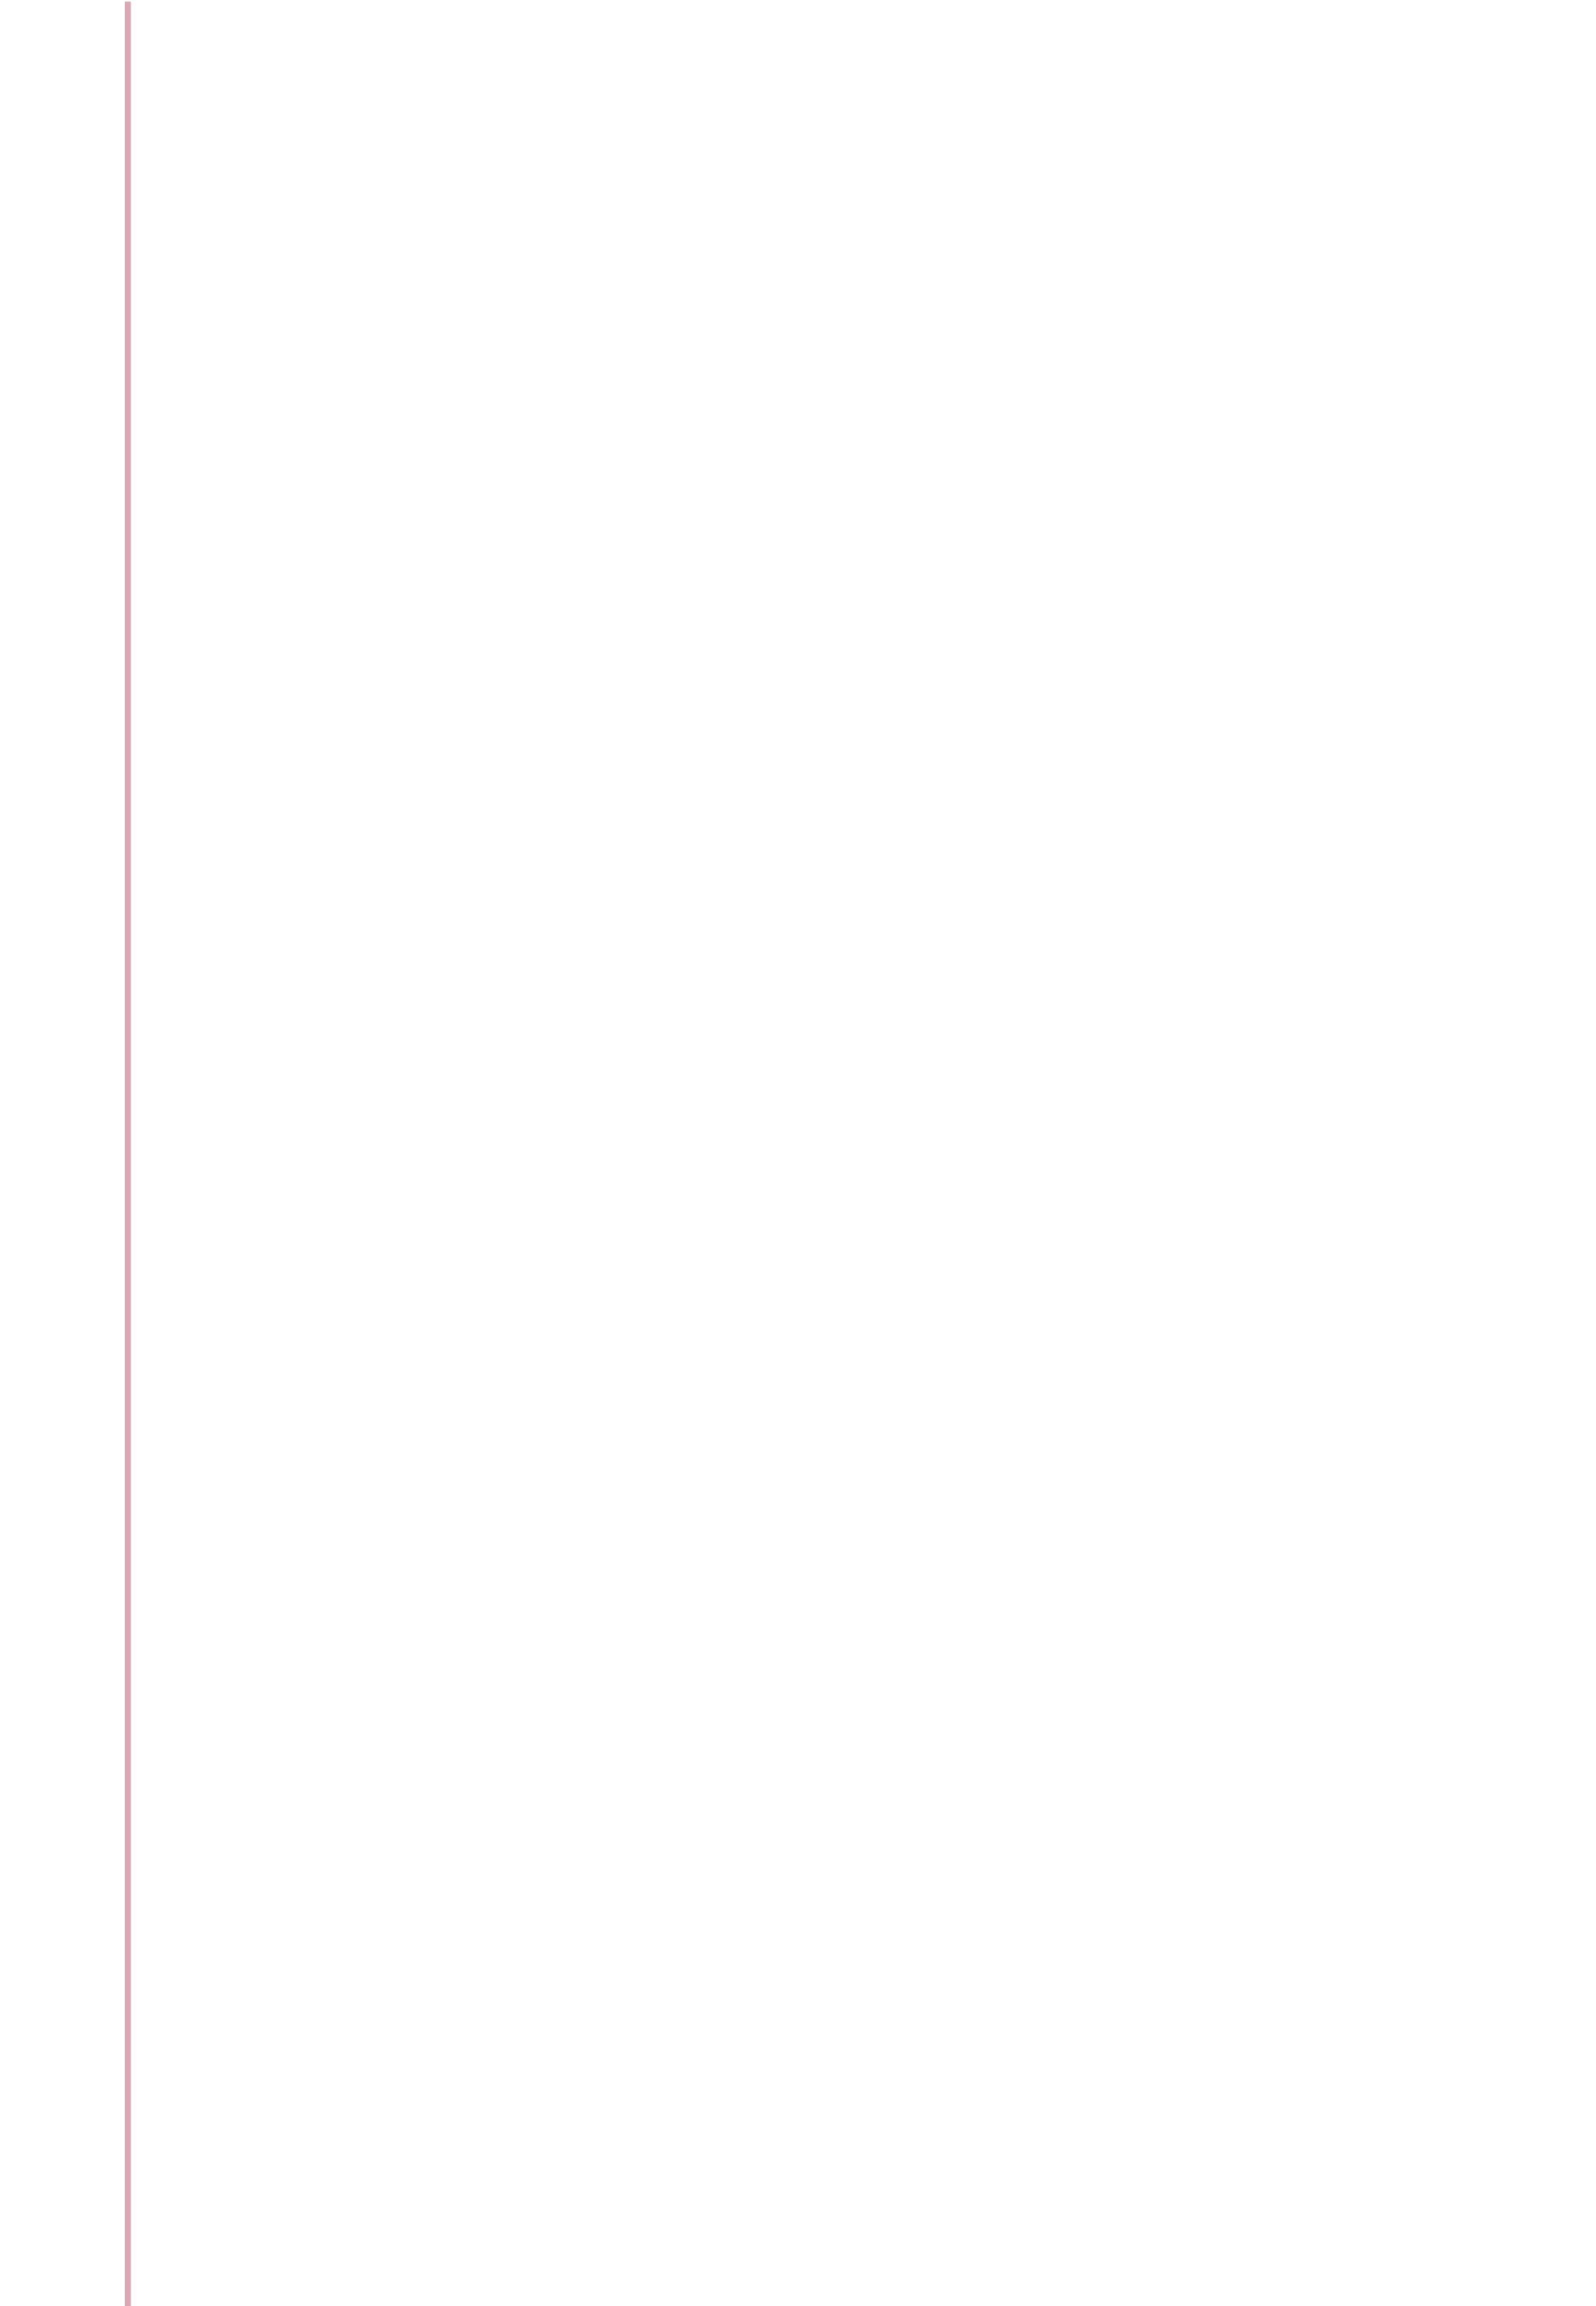
\includegraphics[width=\paperwidth,height=\paperheight]{\_extensions/anu-report/assets/images/page-background.jpg}}


\floatplacement{table}{H}
\renewcommand*\contentsname{차례}
{
\setcounter{tocdepth}{2}
\tableofcontents
}

\mainmatter
\section{일반 현황 -- 통합소득 평균 4,123만원(2.2\%↑) 중위값
2,887만원(4.1\%↑)}\label{uxc77cuxbc18-uxd604uxd669-uxd1b5uxd569uxc18cuxb4dd-uxd3c9uxade0-4123uxb9ccuxc6d02.2-uxc911uxc704uxac12-2887uxb9ccuxc6d04.1}

\textbf{1인당 소득증가율 통합 2.2\%, 근로 2.8\%, 종합 2.3\%, 물가상승률
3.6\%에 모두 못미쳐}

국세청이 최근에 국회에 제출한 통합소득, 종합소득, 근로소득 천분위
자료\footnote{국세청의 천분위 소득자료에 대한 분석은
  참여연대경제개혁센터(김상조 2014)가 처음으로 시도한 바 있는데, 당시
  보고서는 2007\textasciitilde2012년 기간까지의 소득 백분위 자료를
  분석한 것으로 과세미달자에 대한 정보가 제외돼 있었다. 2012년 이후
  과세미달자를 포함한 천분위 소득자료가 국회로 제출되기 시작했으며, 20대
  국회에서 서형수 의원이 2012\textasciitilde2016년 기간의
  통합-근로-종합소득 천분위 자료에 대한 분석결과를 정책보고서로 발간한
  바 있다(서형수의원실 2018). 이후 소득주도성장특위에서 2017년 이후의
  2020년까지의 소득천분위 자료에 대한 분석결과를 제시한 바
  있는데(소득주도성장특별위원회 2022), 이 글은 서형수
  의원실(2012\textasciitilde2016)과
  소득주도성장특위(2017\textasciitilde2020)에서 정리한 자료에
  2021\textasciitilde2023년 자료를 추가로 통합하여 분석한 결과이다.}를
분석한 결과, 2023년 귀속분 근로소득자는 20,852천명, 종합소득 신고자는
11,481천명이었음. 근로소득과 종합소득의 중복 신고인원 5,446천명을
1인으로 합산한 통합소득 인원은 26,888천명이었음.

\begin{figure}

\caption{\label{fig-first1}국세청 천분위 소득자료 포괄대상(2023년)}

\centering{

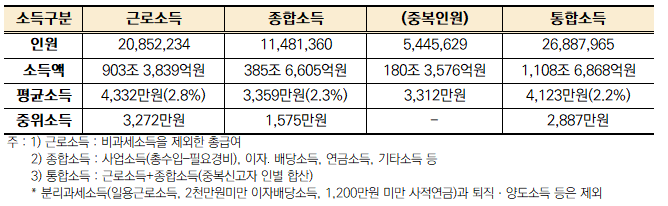
\includegraphics{image/first.png}

}

\end{figure}%

통합소득 총액은 1,108.7조로 전년대비 4.7\% 증가하였으나 소득자 수가
2.5\% 증가하여 1인당 평균소득은 4,123만원 2.2\% 증가에 그치고 중위소득은
2,887만원으로 전년대비 4.1\% 증가하였음. 이러한 낮은 평균소득 증가율은
2023년 연간 소비자물가 상승률 3.6\%에 미치지 못하는 것으로 실질소득은
마이너스 증가에 그친 것을 의미함

\begin{itemize}
\item
  근로소득은 총액 903조 3,839억원으로 1인당 평균 근로소득은
  4,332만원으로 2.8\% 증가하였으며 중위값은 3,272만원으로 4.4\% 증가한
  것으로 나타남
\item
  종합소득은 매출액 기준으로는 1,538조 1,312억원에 달했으나 필요경비를
  차감한 종합소득 금액은 총 385억 6,605억원이었음. 이에 1인당 평균
  종합소득액은 3,359만원으로 전년대비 2.3\% 증가에 그쳤고 중위소득은
  1,575만원으로 9.0\% 증가한 것으로 나타남
\end{itemize}

\begin{figure}

\caption{\label{fig-inc}전년 대비 소득증가율}

\centering{

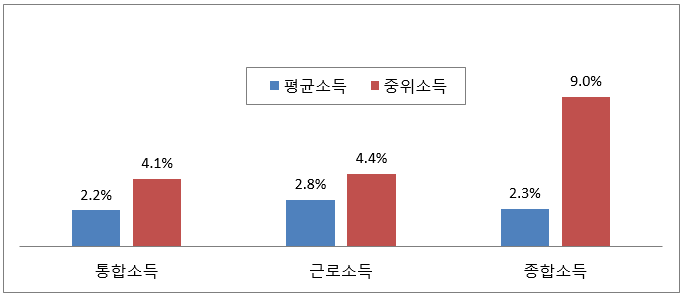
\includegraphics{image/inc.png}

}

\end{figure}%

\begin{figure}

\caption{\label{fig-pinc}소득자수 증감}

\centering{

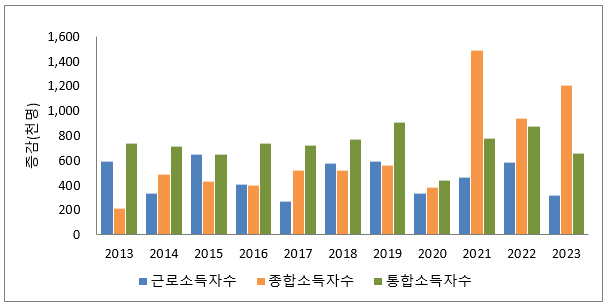
\includegraphics{image/pinc.png}

}

\end{figure}%

\begin{itemize}
\tightlist
\item
  소득신고자 수에 있어서는 전년대비 근로소득자는 313천명 증가(1.5\%),
  종합소득자는 1,206천명(11.7\%), 통합소득자는 657천명(2.5\%) 각각 증가
  ⇒ 종합소득자의 증가규모와 증가율이 매우 높은 상황. 플랫폼특고,
  프리랜서 형태의 고용증가와 N잡러 증가의 영향
\end{itemize}

\section{소득증가율 2018\textasciitilde19년 vs.~2020년 이후 양상 확연히
달라져}\label{uxc18cuxb4dduxc99duxac00uxc728-201819uxb144-vs.-2020uxb144-uxc774uxd6c4-uxc591uxc0c1-uxd655uxc5f0uxd788-uxb2ecuxb77cuxc838}

백분위를 구분하여 전년 대비 통합소득 증가율을 비교하면
2019\textasciitilde19년 시기와 2020년 이후 시기가 확연히 달리짐

\begin{figure}

\caption{\label{fig-means}가장 소득증가율이 가장 높았던 계층과
소득증가율 분포}

\begin{minipage}{\linewidth}

\subcaption{\label{fig-2018}2018년}

\centering{

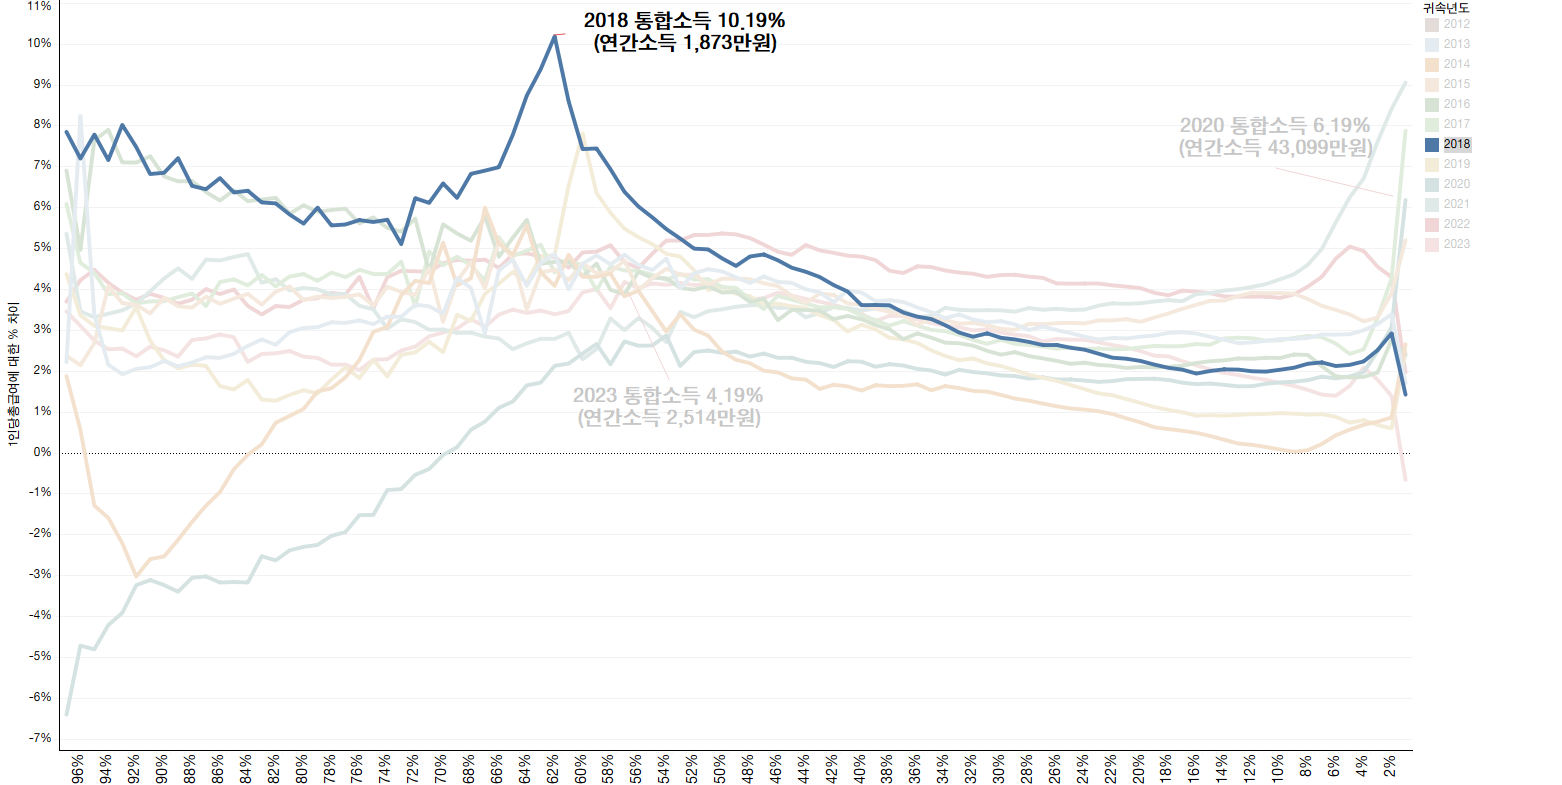
\includegraphics[width=\textwidth,height=2.60417in]{image/2018_100.png}

}

\end{minipage}%
\newline
\begin{minipage}{\linewidth}

\subcaption{\label{fig-2020}2020년}

\centering{

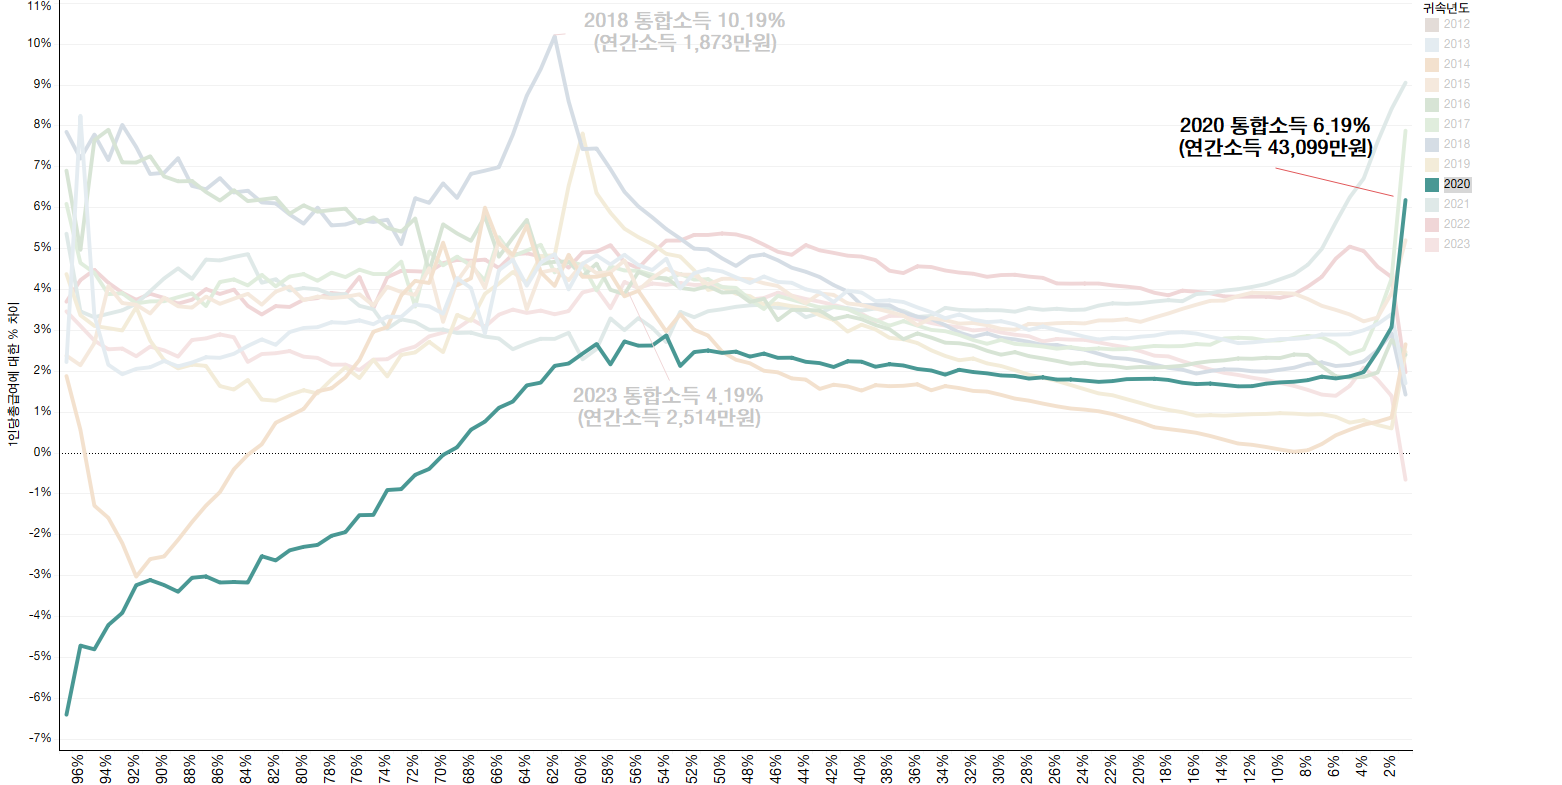
\includegraphics[width=\textwidth,height=2.60417in]{image/2020_100.png}

}

\end{minipage}%
\newline
\begin{minipage}{\linewidth}

\subcaption{\label{fig-2023}2023년}

\centering{

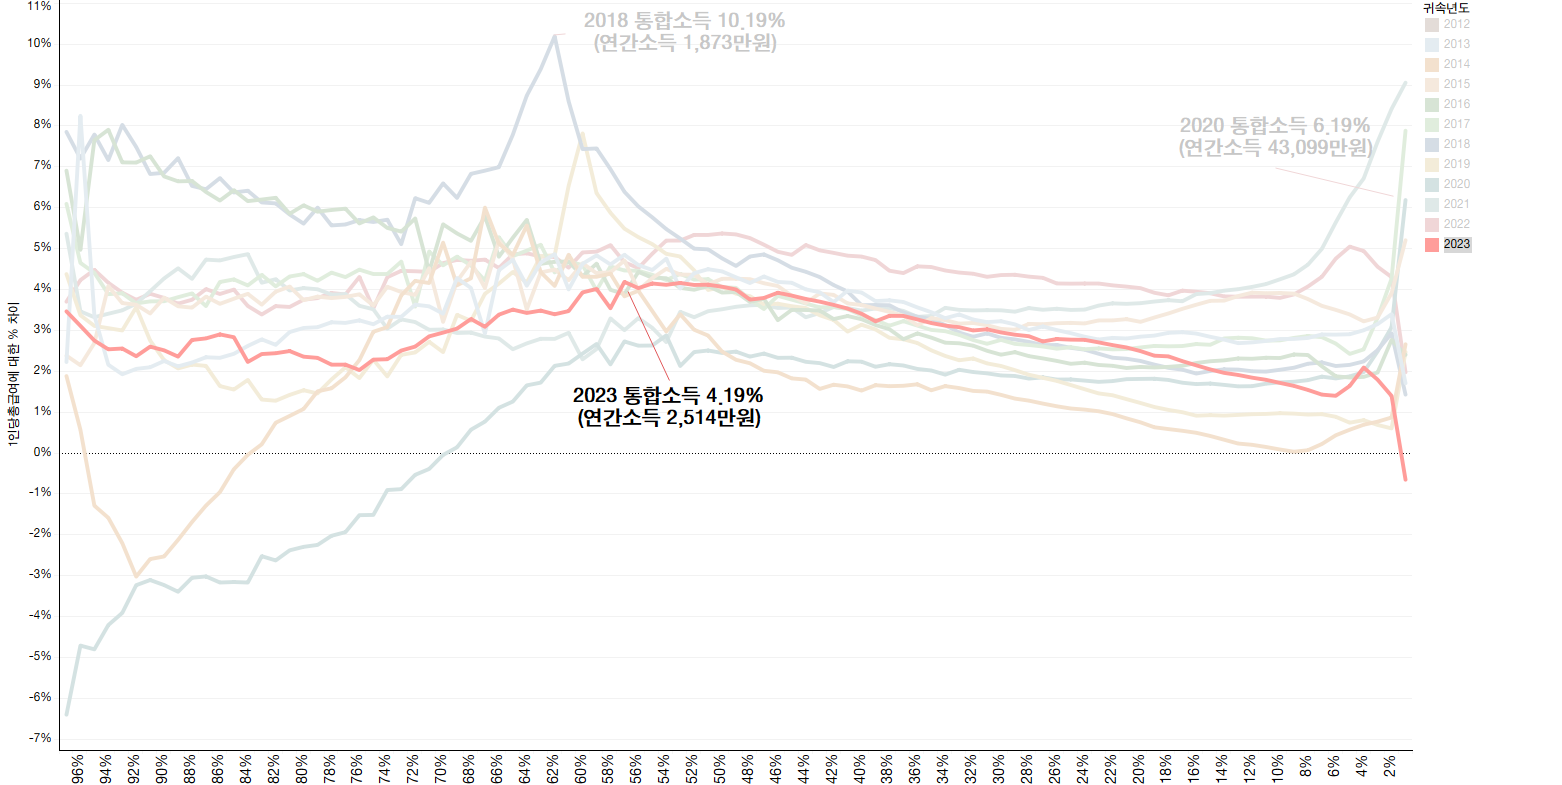
\includegraphics[width=\textwidth,height=2.60417in]{image/2023_100.png}

}

\end{minipage}%

\end{figure}%

\begin{itemize}
\tightlist
\item
  2018년에는 1,873만원 연소득자(하위38분위)의 소득증가율이 10.2\%에 두
  자리에 달했고 사상 최고 수준의 증가율을 기록. 이 해의 최저임금이
  전녀대비 16.4\% 인상된 시급 7,530원으로 월급기준 157만원이었으며,
  연간총액으로 1,889만원으로 거의 정확히 최저임금 수준 소득자의 증가율이
  가장 높은 해였음
\item
  2020년에는 상위1\%에 해당하는 연소득 4억3,099만원 소득자의 증가율이
  6.2\%로 가장 높았지만 하위50\% 이하로 갈수록 소득증가율이 낮아지는
  정반대 현상이 나타났음. 최저임금 인상률은 2.87\%에 그쳤고 최저임금
  수준(연간 2,154만원) 연소득자의 소득증가율은 2.7\%에 불과했음
\item
  2023년에는 연소득 2,514만원 소득자(하위43분위)의 소득증가율이 4.19\%로
  가장 높기는 했고 이들이 최저임금 연소득자(2,413만원)에 해당되는
  계층이었으나 전반적으로 소득증가율이 낮아진 상황
\end{itemize}

최근 수년 간 과정을 보면 최저임금이 높게 인상된 해에는 최저임금
수준(통합소득 분위로는 하위30\% 수준)의 소득자 증가율이 높았고,
최저임금이 낮게 인상된 해에는 해당 계층의 소득증가율이 매우 낮은
증가율을 보임. 최저임금 인상률이 크게 낮아지고 경제상황이 악화되면서
저소득 계층의 소득증가율이 낮아지는 모습을 보이고 있음.

\section{최상위 평균소득과 경계값 -- 상위10\% 평균 1억 5,179만원, 경계값
8,257만원}\label{uxcd5cuxc0c1uxc704-uxd3c9uxade0uxc18cuxb4dduxacfc-uxacbduxacc4uxac12-uxc0c1uxc70410-uxd3c9uxade0-1uxc5b5-5179uxb9ccuxc6d0-uxacbduxacc4uxac12-8257uxb9ccuxc6d0}

\emph{통합소득 상위1\% (26.8만명) 소득경계값 처음으로 2억원 넘겨,
근로소득은 1억 8천만원}

근로소득과 종합소득을 인별로 합산한 통합소득 기준 최상위0.1\%의
평균소득은 17억 3,681만원이며, 상위1\%는 4억 7,619만원, 상위5\%는 2억
78만원, 상위10\%는 1억 5,317만원, 상위20\%는 1억 1,144만원의 평균소득
수준을 보였음

\begin{itemize}
\item
  상위0.1\%에 속하기 위한 소득경계값은 11억 6,905만원이었으며, 상위1\%에
  속하기 위해서는 2억 249만원, 상위5\%는 1억 1,211만원을 넘어야 했음.
  상위10\%의 소득경계값은 8,402만원이고 상위20\%에 속하기 위해서는
  5,850만원을 넘어야 함
\item
  근로소득의 경우 상위0.1\%에 들기 위해서는 6억 9,051만원이 넘어야 했고,
  상위 1\%는 1억 8,014만원, 상위5\%는 1억 1,172만원이 넘어야 함.
  상위10\%는 8,650만원을 넘어야 하고, 상위20\%는 6,248만원을 넘어야 함
\item
  종합소득은 편차가 심해 최상위 0.1\%는 18억 4,657만원이 넘어야 했고
  상위1\%도 2억 5,871만원, 상위5\%도 1억 542만원을 넘겨야 함. 상위10\%는
  6,673만원을 넘어야 했는데, 종합소득자의 상위20\% 경계값는
  3,919만원으로 경계값이 매우 낮음
\end{itemize}

\begin{figure}

\caption{\label{fig-mean}상위소득계층 평균소득과
경계값(2012\textasciitilde2023)}

\begin{minipage}{\linewidth}

\subcaption{\label{fig-mean1}통합소득}

\centering{

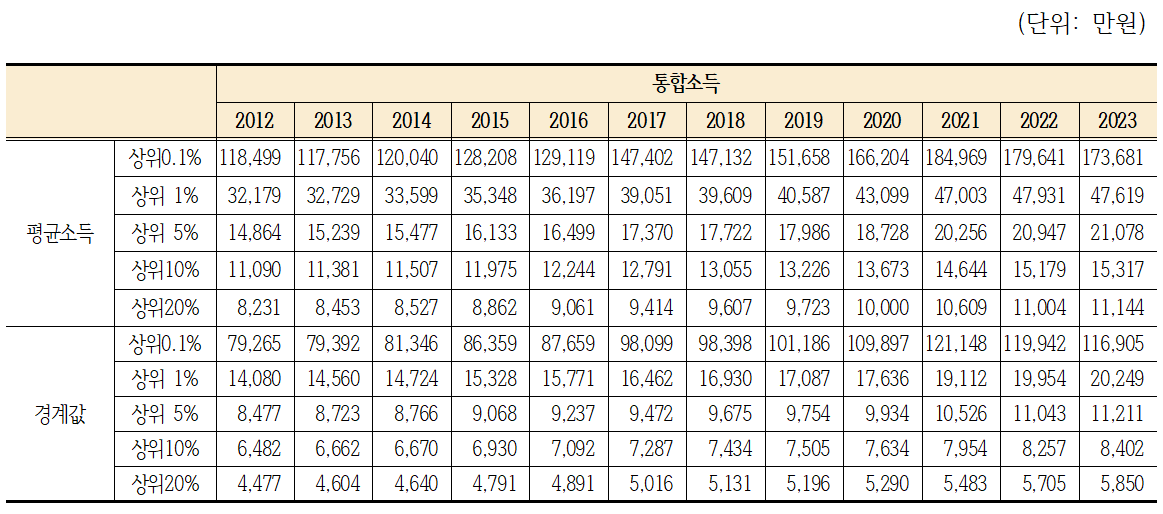
\includegraphics{image/means1.png}

}

\end{minipage}%
\newline
\begin{minipage}{\linewidth}

\subcaption{\label{fig-mean2}근로소득}

\centering{

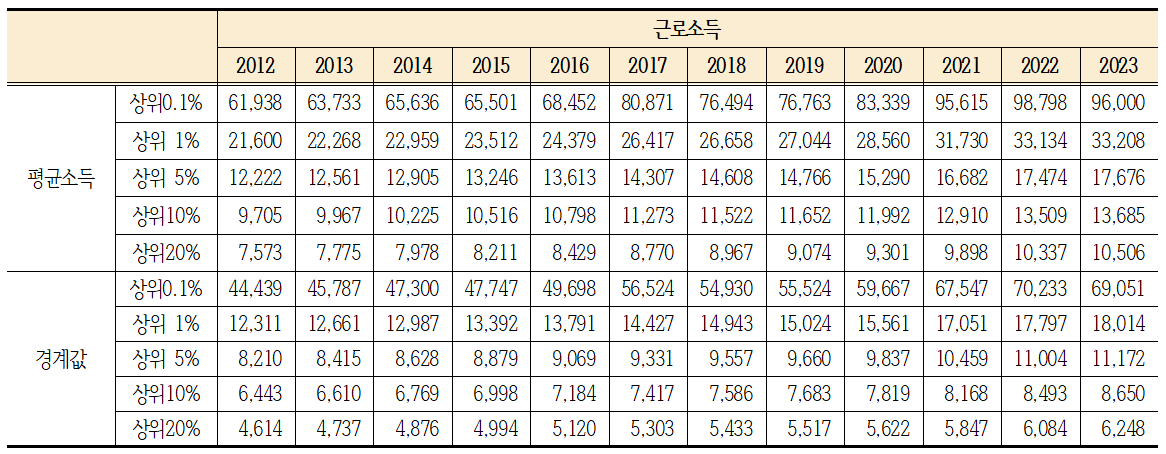
\includegraphics{image/means2.png}

}

\end{minipage}%
\newline
\begin{minipage}{\linewidth}

\subcaption{\label{fig-mean3}종합소득}

\centering{

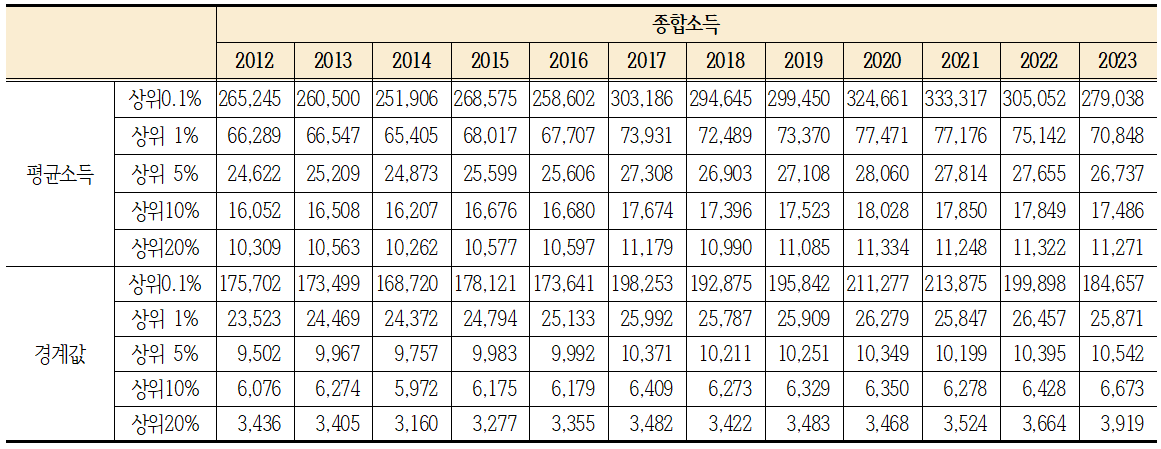
\includegraphics{image/means3.png}

}

\end{minipage}%

\end{figure}%

\section{소득집중도 - 최근 2년 개선에도 여전히 코로나 때보다 높고 2019년
수준 회복
못해}\label{uxc18cuxb4dduxc9d1uxc911uxb3c4---uxcd5cuxadfc-2uxb144-uxac1cuxc120uxc5d0uxb3c4-uxc5ecuxc804uxd788-uxcf54uxb85cuxb098-uxb54cuxbcf4uxb2e4-uxb192uxace0-2019uxb144-uxc218uxc900-uxd68cuxbcf5-uxbabbuxd574}

상위10\%가 통합소득 37.1\%. 근로소득 31.6\%, 종합소득 52.1\% 차지*

2017\textasciitilde2019년 기간 동안 상위 소득계층의 소득비중은
지속적으로 축소돼 왔으나, 코로나위기 발발로 2020\textasciitilde21년
상위층 소득점유비중이 다시 크게 증가. 2022\textasciitilde2023년에는 다시
2년 연속 상위소득 점유비중이 하락하고 있으나 2020년 코로나 때보다 높은
수준

\begin{itemize}
\item
  통합소득 상위10\% 점유비중은 2017년 37.2\%, 2018년 36.8\%, 2019년
  36.6\%로 2년 연속 하락하다 2020년 37.0\%, 2021년 37.8\%로 2년 연속
  증가했으며, 2022\textasciitilde2023년에 37.6\%, 37.1\%로 다시 완화
  추세

  \begin{itemize}
  \tightlist
  \item
    2023년 상위10\% 소득점유비중(37.1\%)은 2020년(36.6\%) 코로나 때보다
    높은 수준이며, 소득집중도가 가장 낮았던 2019년(39.6\%) 수준은 회복
    못한 상태
  \end{itemize}
\item
  근로소득은 2017\textasciitilde2019년 동안 상위10\% 점유비중이 연속
  하락(32.0\% → 31.6\% → 31.1\%)했으나 코로나19 발발 이후
  2020\textasciitilde2021년 연속 상승한 뒤 2022\textasciitilde2023년
  다시 하락

  \begin{itemize}
  \tightlist
  \item
    근로소득 상위10\% 점유비중 31.1\%('19년) → 31.3\%('20년) →
    32.1\%('21년) → 32.1\%('22년) → 31.6\%('23년)
  \end{itemize}
\item
  종합소득도 2018\textasciitilde2019년 연속 하락(56.5\% → 56.3\% →
  55.9\%)했으나 2020년에 56.9\%로 크게 상승한 뒤
  2021\textasciitilde2022년 3년 연속 하락. 자영업자는 2020년 한 해만
  소득집중도 상승

  \begin{itemize}
  \tightlist
  \item
    종합소득 상위10\% 점유비중 56.0\%('19년) → 56.9\%('20년) →
    55.7\%('21년) → 54.3\%('22년) → 52.1\%('23년)
  \end{itemize}
\end{itemize}

\begin{figure}

\caption{\label{fig-cons}상위10\% 소득 점유비중 추이(2017-2023)}

\begin{minipage}{0.33\linewidth}

\subcaption{\label{fig-cons1}통합소득}

\centering{

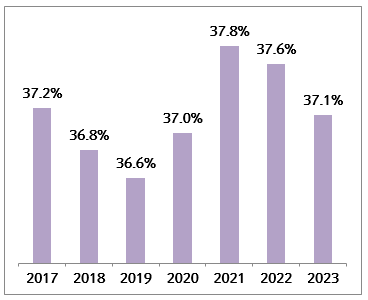
\includegraphics{image/cons1.png}

}

\end{minipage}%
%
\begin{minipage}{0.33\linewidth}

\subcaption{\label{fig-cons2}근로소득}

\centering{

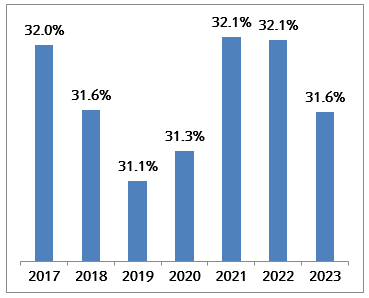
\includegraphics{image/cons2.png}

}

\end{minipage}%
%
\begin{minipage}{0.33\linewidth}

\subcaption{\label{fig-cons3}종합소득}

\centering{

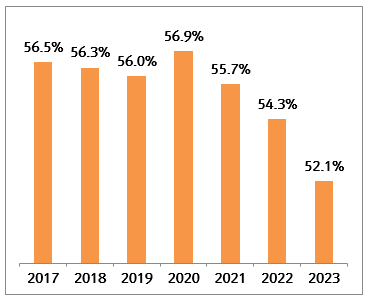
\includegraphics{image/cons3.png}

}

\end{minipage}%

\end{figure}%

최상위 0.1\% 및 1\%, 5\% 소득비중과 상위20\% 소득비중도
2017\textasciitilde2019년 빠르게 하락하다가 2020\textasciitilde2021년
코로나 발발 이후 모두 증가하여 소득집중도 심화.
2022\textasciitilde2023년에는 소득집중도 다소 하락

\begin{itemize}
\item
  통합소득 상위0.1\%, 상위1\%, 상위5\% 소득비중은
  2017\textasciitilde2019년 기간 동안 --0.1\%p, -0.1\%p, -0.4\%p
  하락했으나 2019\textasciitilde2021년 기간 동안에는 +0.6\%p, +0.9\%p,
  +1.3\%p 증가하여 2017년 수준보다 악화된 상태로 회귀

  \begin{itemize}
  \tightlist
  \item
    2021\textasciitilde203년 기간 동안에는 --0.6\%p, -0.6\%p, -0.6\%p
    다시 하락. 최상위0.1\%는 2019년 수준으로 회복했으나 상위1\%, 상위5\%
    소득점유 비중은 2019년보다 나쁜 상태
  \end{itemize}
\item
  근로소득 상위0.1\%, 상위1\%, 상위5\% 소득비중은
  2017\textasciitilde2019년 기간 동안 --0.2\%p, -0.3\%p, -0.6\%p
  하락했으나 2019\textasciitilde2021년 기간 동안 +0.3\%p, +0.7\%p,
  +1.0\%p 증가하여 2017년 수준보다 악화. 2021\textasciitilde2023년
  --0.2\%p, -0.2\%p, -0.3\%p 다시 하락헸으나 2019년 수준 회복 못한 상태
\item
  종합소득은 상위1\%, 상위5\% 소득비중이 2020년 한해 동안만 증가한 뒤에
  2020\textasciitilde2021년 기간 동안 연속 하락했고, 최상위0.1\%
  점유비중도 2020년, 2021년 2년 연속 증가하기는 했으나 2022년과 2023년에
  큰 폭으로 2년 연속(-0.9\%p, -1.0\%p) 다시 하락해 2017년 수준보다
  전체적으로 상위소득계층 비중이 감소한 것으로 나타남

  \begin{itemize}
  \tightlist
  \item
    자영업와 개인사업자의 최상위층 소득비중은 코로나와 경기상황 등의
    영향으로 전체적으로 감소한 것으로 나타남
  \end{itemize}
\end{itemize}

\begin{figure}

\caption{\label{fig-cocons}소득계층별 점유비중 추이(2017-2023)}

\centering{

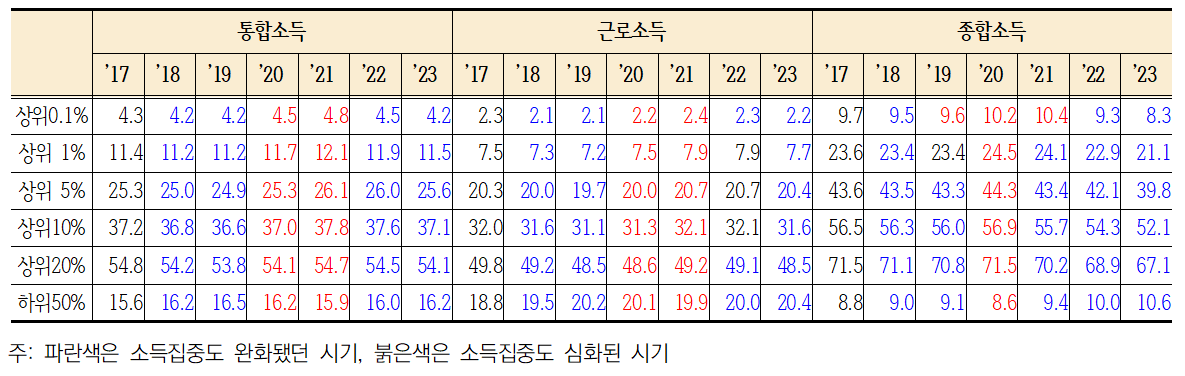
\includegraphics{image/cocons.png}

}

\end{figure}%

\section{소득분배지표 -- 코로나위기 이후 악화되었던 소득분배지표도 2년
연속
개선}\label{uxc18cuxb4dduxbd84uxbc30uxc9c0uxd45c-uxcf54uxb85cuxb098uxc704uxae30-uxc774uxd6c4-uxc545uxd654uxb418uxc5c8uxb358-uxc18cuxb4dduxbd84uxbc30uxc9c0uxd45cuxb3c4-2uxb144-uxc5f0uxc18d-uxac1cuxc120}

5분위배율과 팔마비율 등 분배지표\footnote{국세청 소득자료는 상위층
  소득의 정확성은 높으나 하위층 소득의 정확도가 낮고 변동성이 많아
  하위소득층 포괄범위가 좁은 10분위배율 대신 5분위배율 또는 팔마비율을
  사용}는 2017-2019년 기간 동안은 크게 개선되어 2019년 통합소득
분배지표는 국세청이 소득 천분위 자료를 생산하기 시작한 2012년 이후 가장
좋은 최저치를 기록

\begin{itemize}
\tightlist
\item
  5분위배율 최고 26.1('15) → 최저 23.7('19), 팔마비율 최고 4.04('12) →
  최저 3.58('19)
\end{itemize}

그러나 코로나위기 발발 이후 2020\textasciitilde2021년 기간 동안
통합소득과 근로소득 분배지표가다시 악화되었다가
2021\textasciitilde2023년 2년간 다시 개선되었으며. 종합소득 분배지표는
2020년 한해 동안 악화되었다가 2020\textasciitilde2023년 기간 동안 3년
연속 상위소득계층의 소득비중이 감소하면서 개선 추이를 보임

\begin{figure}

\caption{\label{fig-dis1}통합소득 소득분배지표 추이(2012-2023)}

\centering{

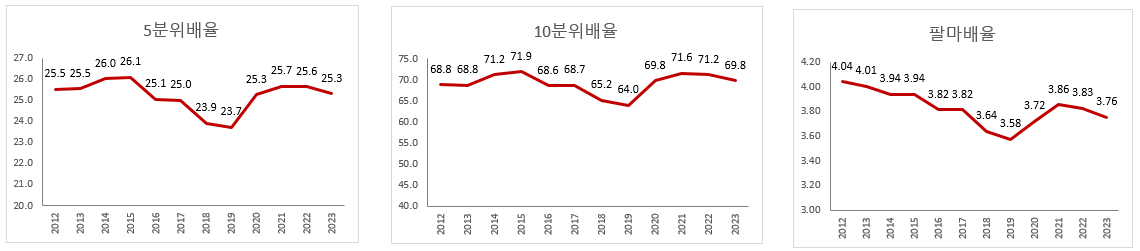
\includegraphics{image/dis1.png}

}

\end{figure}%

\begin{figure}

\caption{\label{fig-dis2}근로소득 소득분배지표 추이(2012-2023)}

\centering{

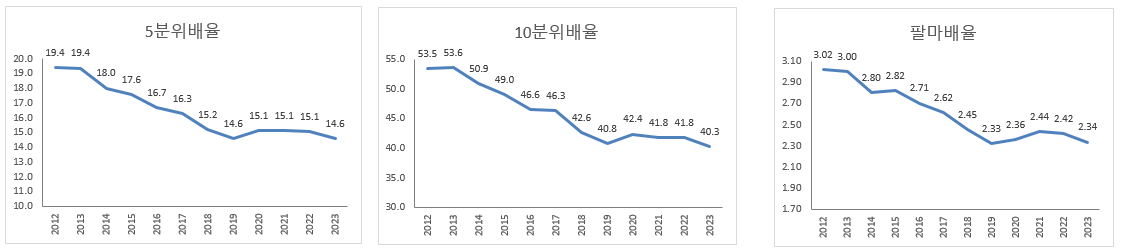
\includegraphics{image/dis2.png}

}

\end{figure}%

\begin{figure}

\caption{\label{fig-dis3}종합소득 소득분배지표 추이(2012-2023)}

\centering{

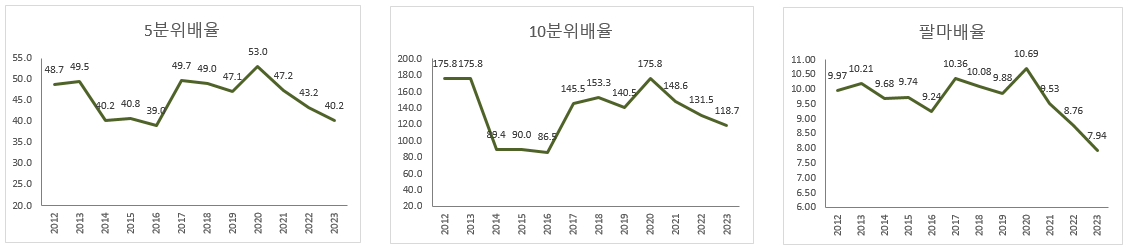
\includegraphics{image/dis3.png}

}

\end{figure}%

\section{고소득층 세율 하락, 조세에 의한 소득분배 개선 효과는
약화}\label{uxace0uxc18cuxb4dduxce35-uxc138uxc728-uxd558uxb77d-uxc870uxc138uxc5d0-uxc758uxd55c-uxc18cuxb4dduxbd84uxbc30-uxac1cuxc120-uxd6a8uxacfcuxb294-uxc57duxd654}

2020\textasciitilde2021년 기간 동안 세전 통합소득 5분위배율과 팔마비율이
크게 상승하고 세후소득 기준 5분위배율과 팔마비율도 악화된 후 2021년 이후
완만한 개선

\begin{itemize}
\item
  2019년 대비 2021년 세전 통합소득 5분위배율과 팔마비율은 각각 1.96배,
  0.28배 증가했으며, 세후 5분위배율과 팔마비율은 각각 1.40배, 0.18배
  증가한 것으로 나타나 세전 소득의 악화보다 세후 소득의 분배지표 악화는
  그보다 덜 악화
\item
  2021년 대비 2023년 세전 통합소득 5분위배율과 팔마비율은 각각 --0.37배,
  -0.10배 개선되었으나 세후 통합소득의 5분위배율과 팔마비율은 각각
  --0.23배, -0.07배 개선되는데 그쳤으며, 통합소득 5분위배율의 세전소득과
  세후소득간 차이가 2022년 3.4배에서 2023년 3.2배로 줄어들고 팔바비율의
  세전소득과 세후소득간 차이도 2022년 0.64배에서 2023년 0.61배로 조세에
  의한 불평등 개선 효과\footnote{조세효과 = 세전 5분위배율 또는 팔마비율
    -- 세후 5분위배율 또는 팔마비율}가 약화되고 있음
\end{itemize}

\begin{figure}

\caption{\label{fig-dist3_1}통합소득 분배지표와 조세효과}

\centering{

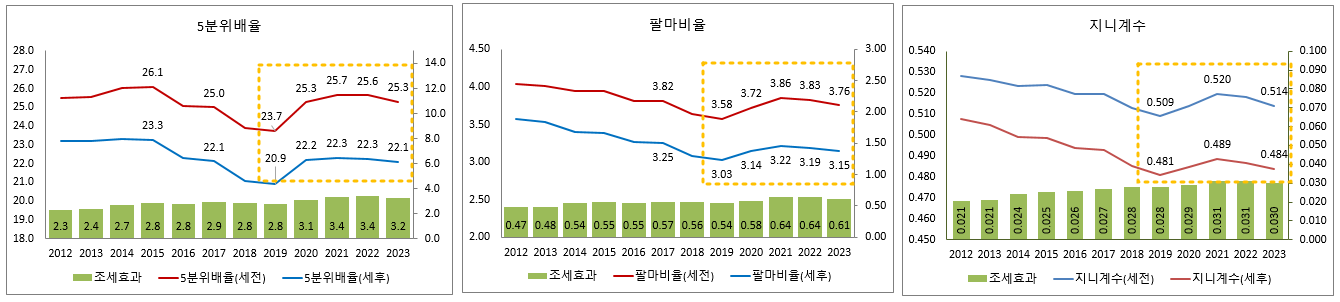
\includegraphics{image/dist3_1.png}

}

\end{figure}%

\begin{figure}

\caption{\label{fig-dist3_2}근로소득 분배지표와 조세효과}

\centering{

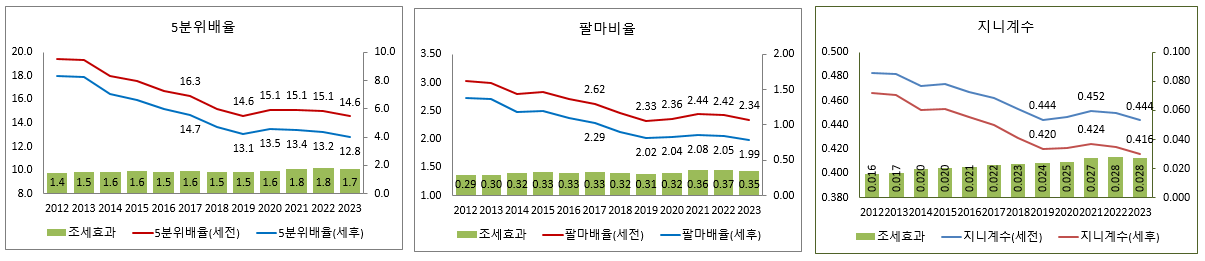
\includegraphics{image/dist3_2.png}

}

\end{figure}%

\begin{figure}

\caption{\label{fig-dist3_3}종합소득 분배지표와 조세효과}

\centering{

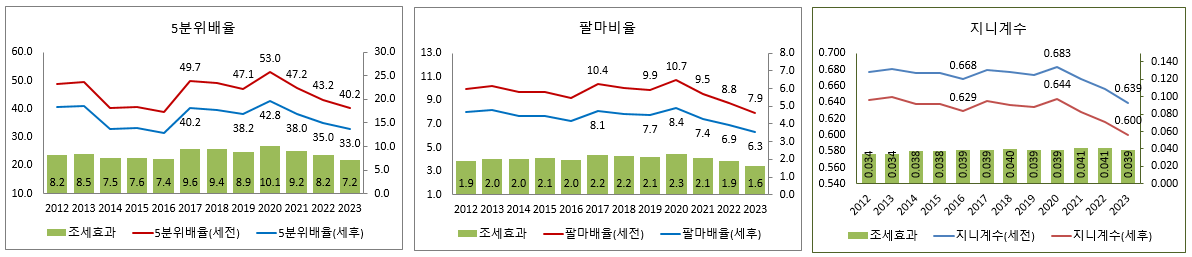
\includegraphics{image/dist3_3.png}

}

\end{figure}%

2020년 이후 코로나로 인해 악화되었던 개인소득 분배가 2021년 이후 다시
개선되고 있는 상황은 긍정적임. 그러나 세전소득과 세후소득의 불평등
차이를 의미하는 조세의 불평등개선 효과는 점차 감소하고 있는 상황임

이와 함께 상위소득 계층의 소득비중이 감소하고 있지만 상위소득층이
소득세를 부담하는 비중도 빠르게 줄어들고 있으며, 2023년 이후 감세정책
등에 의해 이러한 추세가 더 강화될 수 있는 상황임

\begin{itemize}
\item
  통합소득 상위10\%가 전체 소득세에서 부담하는 비중은 2014년 80\%를
  차지했으나 하위90\% 계층의 소득증가와 납세액 증가 등에 의해 2019년에
  77.4\%까지 하락했음. 2022년까지는 평균세율이 상승하는 추세 속에서
  세액비중이 감소하였지만, 2022년 이후에는 평균세율이 하락하면서
  세액비중이 감소하고 있기 때문에 이같은 추세가 지속될 경우 조세에 의한
  불평등 개선효과는 점점 축소될 위험이 있음
\item
  근로소득 상위10\%가 근로소득세에서 부담하는 비중은 2014년 76.8\%를
  차지했으나 2019년까지 72.5\%로 하락했음. 2022년까지는 평균세율이
  상승하는 추세 속에서 세액비중이 감소하였지만 2022년 이후에는
  평균세율이 15.5\%에서 15.1\%로 하락하면서 세액비중이 감소하고 있는
  상황임
\item
  종합소득은 상위10\%가 부담하는 소득세액 비중이 2021년 86.7\%로
  최고치를 기록한 뒤 평균세율과 세액비중이 빠르게 하락하고 있는 상황임
\end{itemize}

향후 소득세의 감세가 추가적으로 추진될 경우 세후 소득의 불평등 개선
효과가 약화되고 세후 소득집중도가 심화될 위험이 있음

\begin{figure}

\caption{\label{fig-cons_tax}상위10\% 계층의 소득세 비중과 평균세율
추이(2012-2023)}

\centering{

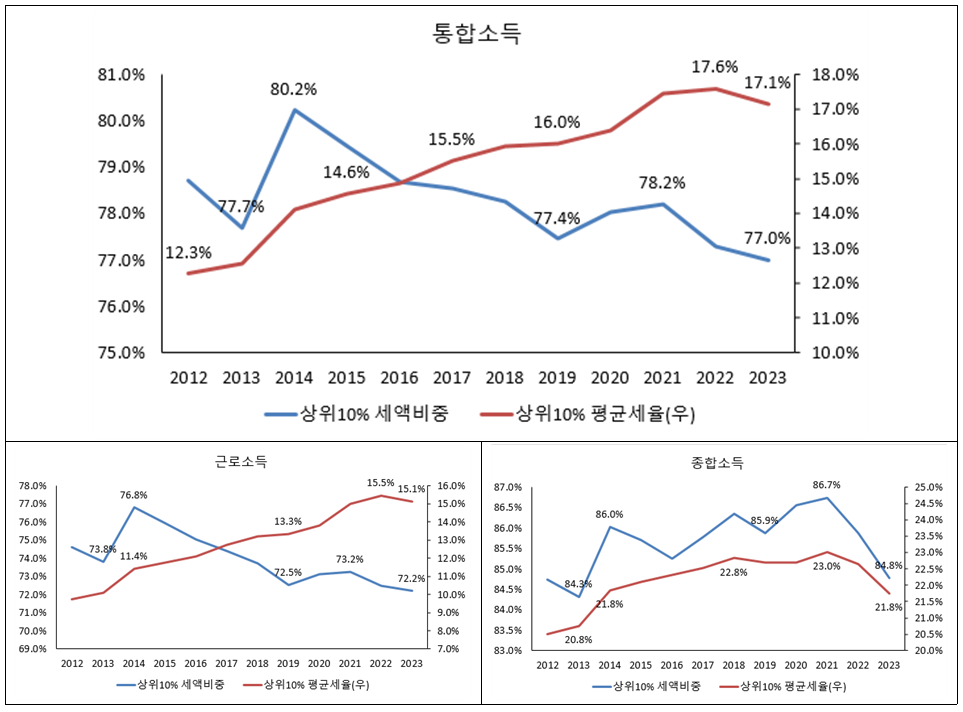
\includegraphics{image/cons_tax.png}

}

\end{figure}%

\section{}\label{section}

\section{평가와 시사점}\label{uxd3c9uxac00uxc640-uxc2dcuxc0acuxc810}

국세청의 통합소득 천분위 자료를 분석한 결과 2022\textasciitilde2023년
기간 동안 2년 연속 소득집중도가 완화되고 분배지표가 개선됨

하지만, 2023년 들어 고소득층의 평균세율이 하락하고 고소득층이 소득세을
부담하는 비중이 하락하면서 조세의 의한 소득분배 개선 효과가 약화되고
있는 상황임

향후 고소득에 대한 추가감세 등이 진행될 경우 조세에 의한 소득분배 개선
효과가 더욱 약화되고 소득집중도가 심화되고 소득분배가 악화될 위험이 있음

\section*{참고문헌}\label{uxcc38uxace0uxbb38uxd5cc}
\addcontentsline{toc}{section}{참고문헌}

\phantomsection\label{refs}
\begin{CSLReferences}{1}{0}
\bibitem[\citeproctext]{ref-gimsangjo2014}
김상조. 2014. {``{국세청의 통합소득 자료를 이용한 소득분배 및 실효세율
추이 분석 : 모집단 기준 전환 100분위 자료를 기초로}.''}
\emph{경제개혁리포트}, June, 1--35.

\bibitem[\citeproctext]{ref-seohyeongsuyiweonsil2018}
서형수의원실. 2018. {``계층별 소득분포와 실효세율 추이 - 2018
기획재정위원회 국정감사 정책자료집.''}

\bibitem[\citeproctext]{ref-sodeugjudoseongjangteugbyeolwiweonhoe2022}
소득주도성장특별위원회. 2022. {``국세청 소득자료를 통해 본 개인소득 분배
상황과 시사점.''}

\end{CSLReferences}


\backmatter


\end{document}
